\paragraph{Model configuration}\mbox{}\\

\begin{table}[H]
\centering
\begin{tabular}{|l|l|}
\hline
\textbf{Parameter} & \textbf{Value} \\
\hline
\multicolumn{2}{|c|}{\textbf{Training}} \\
\hline
Batch Size & 5 \\
\hline
Seed & 42 \\
\hline
Epochs & 15000 \\
\hline
Training Ratio & 0.9 \\
\hline
Number of Nodes & 1 \\
\hline
Number of Devices & 1 \\
\hline
Device & CUDA \\
\hline
Float precision & 32 \\
\hline
Metric to Monitor & val/loss \\
\hline
Metric Mode & Min \\
\hline
\multicolumn{2}{|c|}{\textbf{Model}} \\
\hline
Learning Rate & 0.0001 \\
\hline
Loss Type & L1 \\
\hline
VQGAN Checkpoint Path & ./models/meta_vqgan/checkpoints/meta_vqgan-v5.ckpt \\
\hline
Probability of Focus Present & 0.0 \\
\hline
Gradient Scaler Enabled & False \\
\hline
Focus Present Mask & Null \\
\hline
Max Gradient Norm & Null \\
\hline
\multicolumn{2}{|c|}{\textbf{EMA Configuration}} \\
\hline
Decay & 0.995 \\
\hline
Start Step & 2000 \\
\hline
Update Every Step & 10 \\
\hline
\multicolumn{2}{|c|}{\textbf{Scan Parameters}} \\
\hline
Image Size & 64 \\
\hline
Depth Size & 16 \\
\hline
Number of Channels & 8 \\
\hline
\multicolumn{2}{|c|}{\textbf{Scheduler Parameters}} \\
\hline
Timesteps & 300 \\
\hline
\multicolumn{2}{|c|}{\textbf{UNet Parameters}} \\
\hline
Dimension Multipliers & [1, 2, 4, 8] \\
\hline
\multicolumn{2}{|c|}{\textbf{Dataset Configuration}} \\
\hline
Caching & Disk \\
\hline
Path & /ravana/d3d_work/micorl/data/ct_images_prostate_32fixed/ \\
\hline
Image Size & 128 \\
\hline
Number of Slices & 32 \\
\hline
Window Width & 400 \\
\hline
Window Level & 60 \\
\hline
\end{tabular}
\caption{Parameters for the Meta Diffuser}
\label{table:meta_diffuser_params}
\end{table}



\paragraph{Training}\mbox{}\\
\begin{figure}[H]
\minipage{0.49\textwidth}
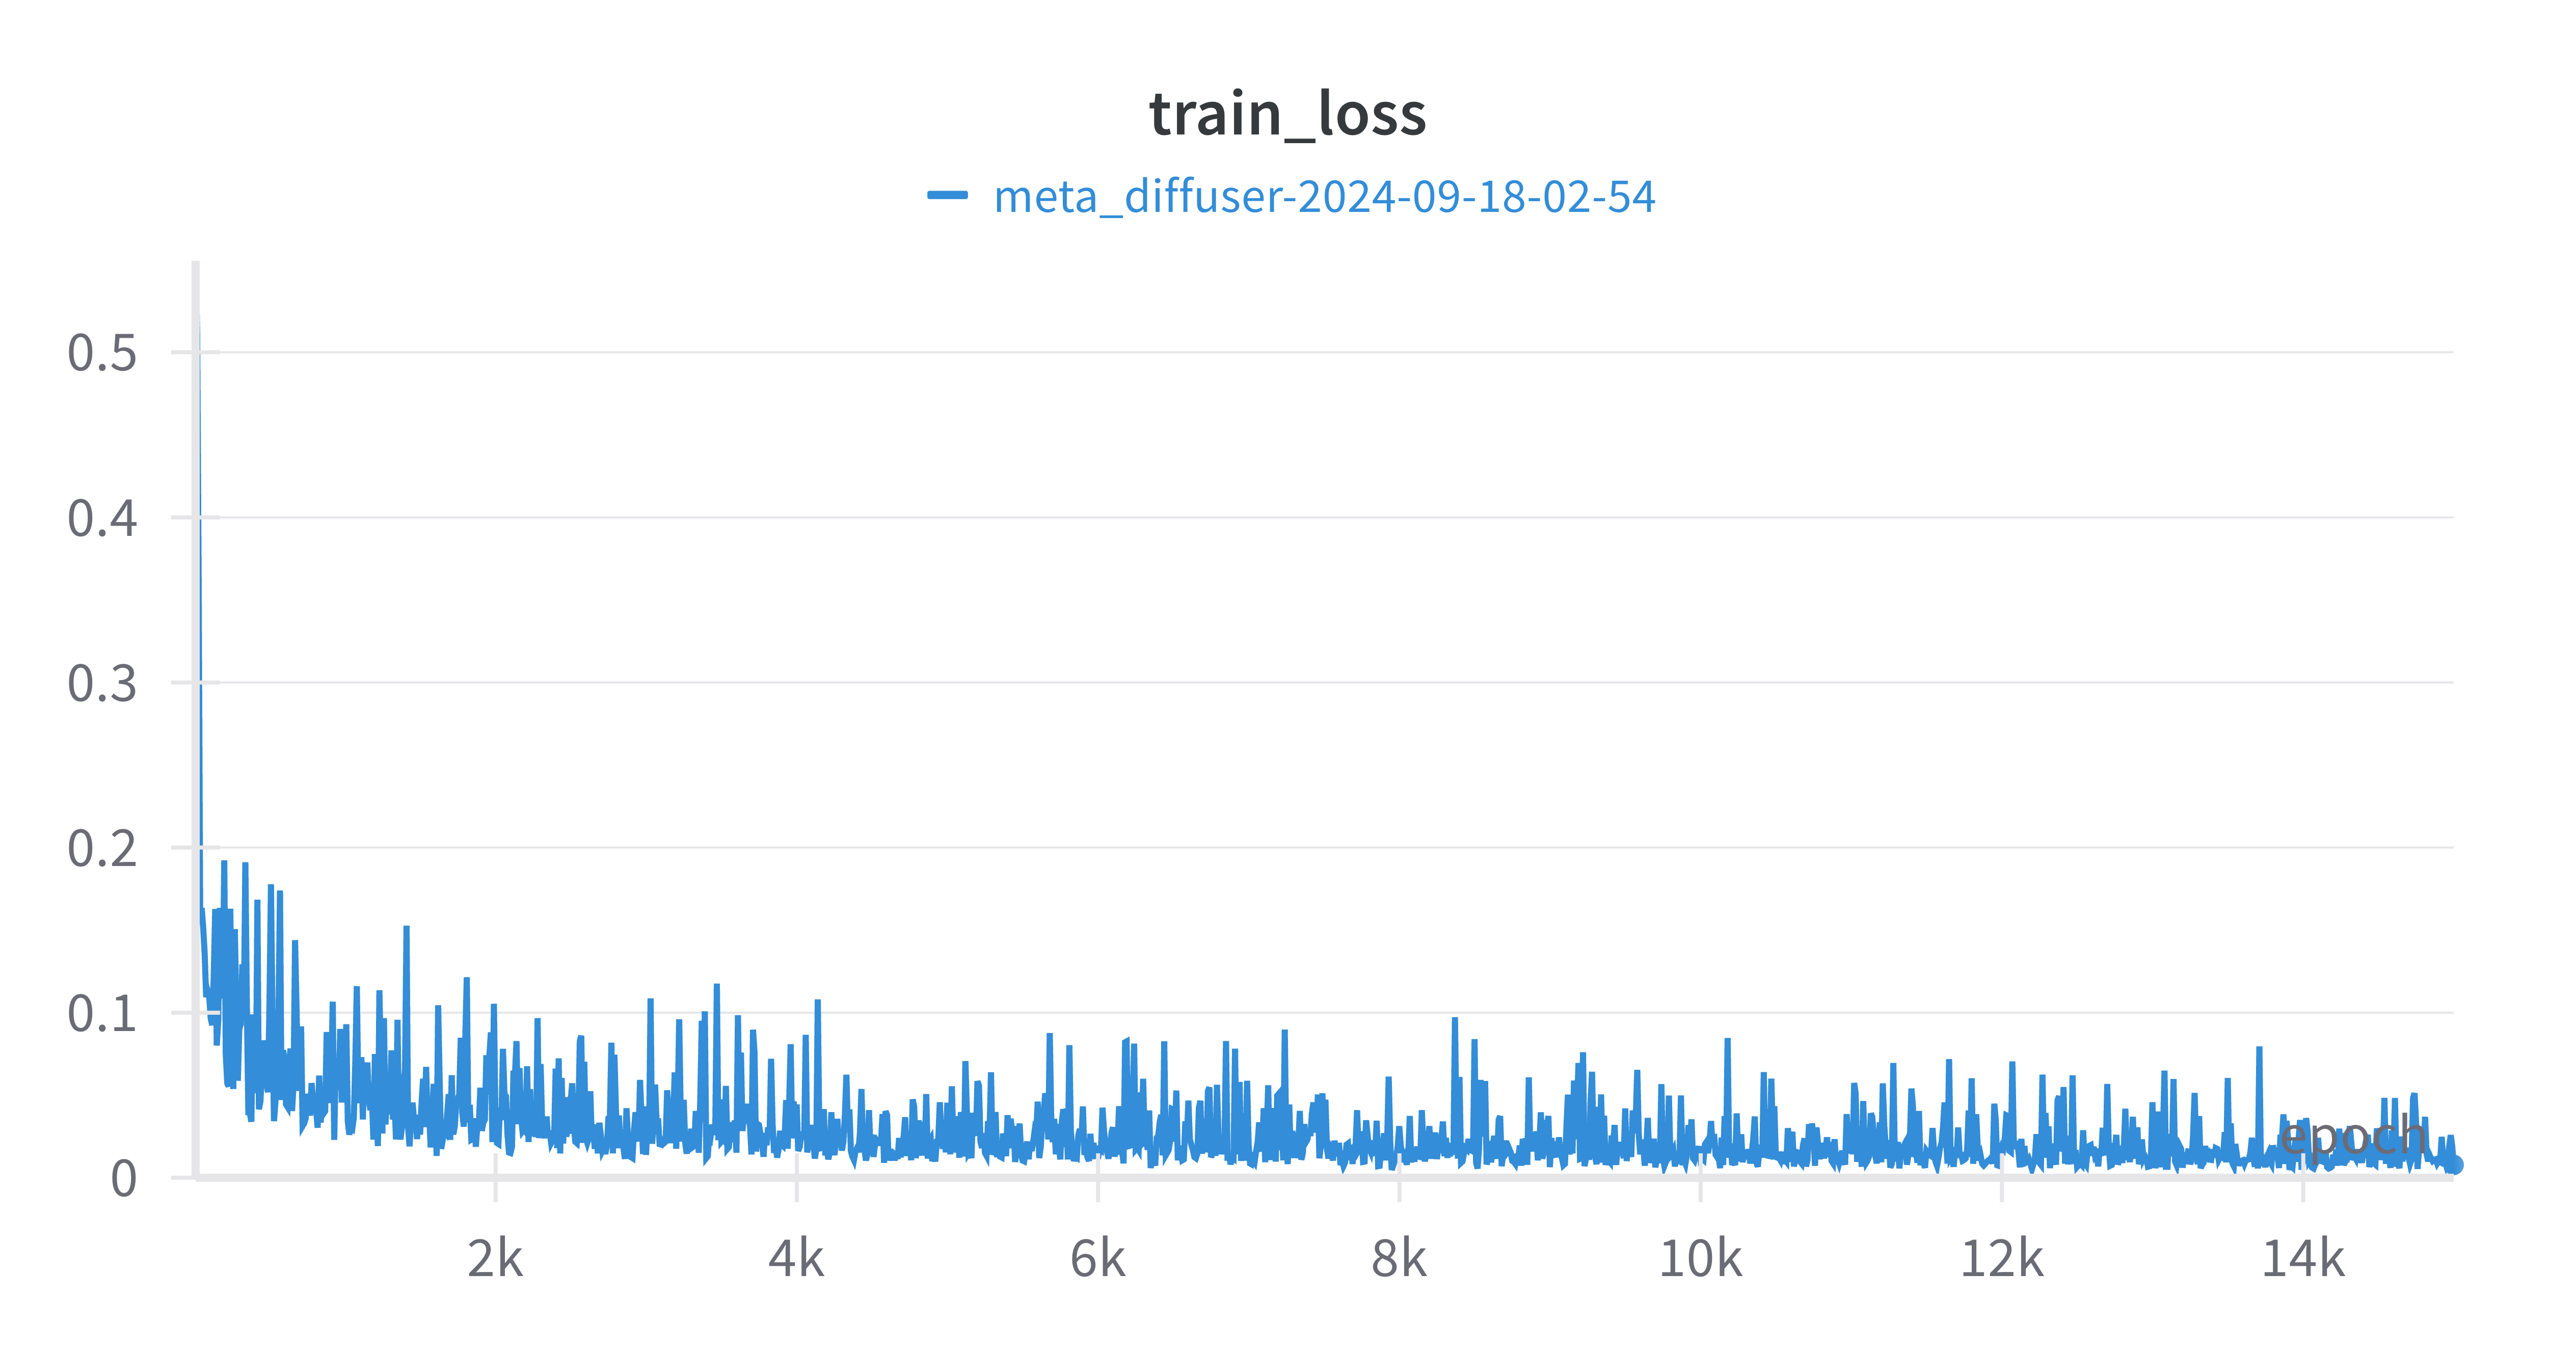
\includegraphics[width=\linewidth]{detailed_engineering/Meta Diffusion/charts/train_loss.png}
\caption{Loss during the training. Lower is better.}
\endminipage\hfill
\minipage{0.49\textwidth}
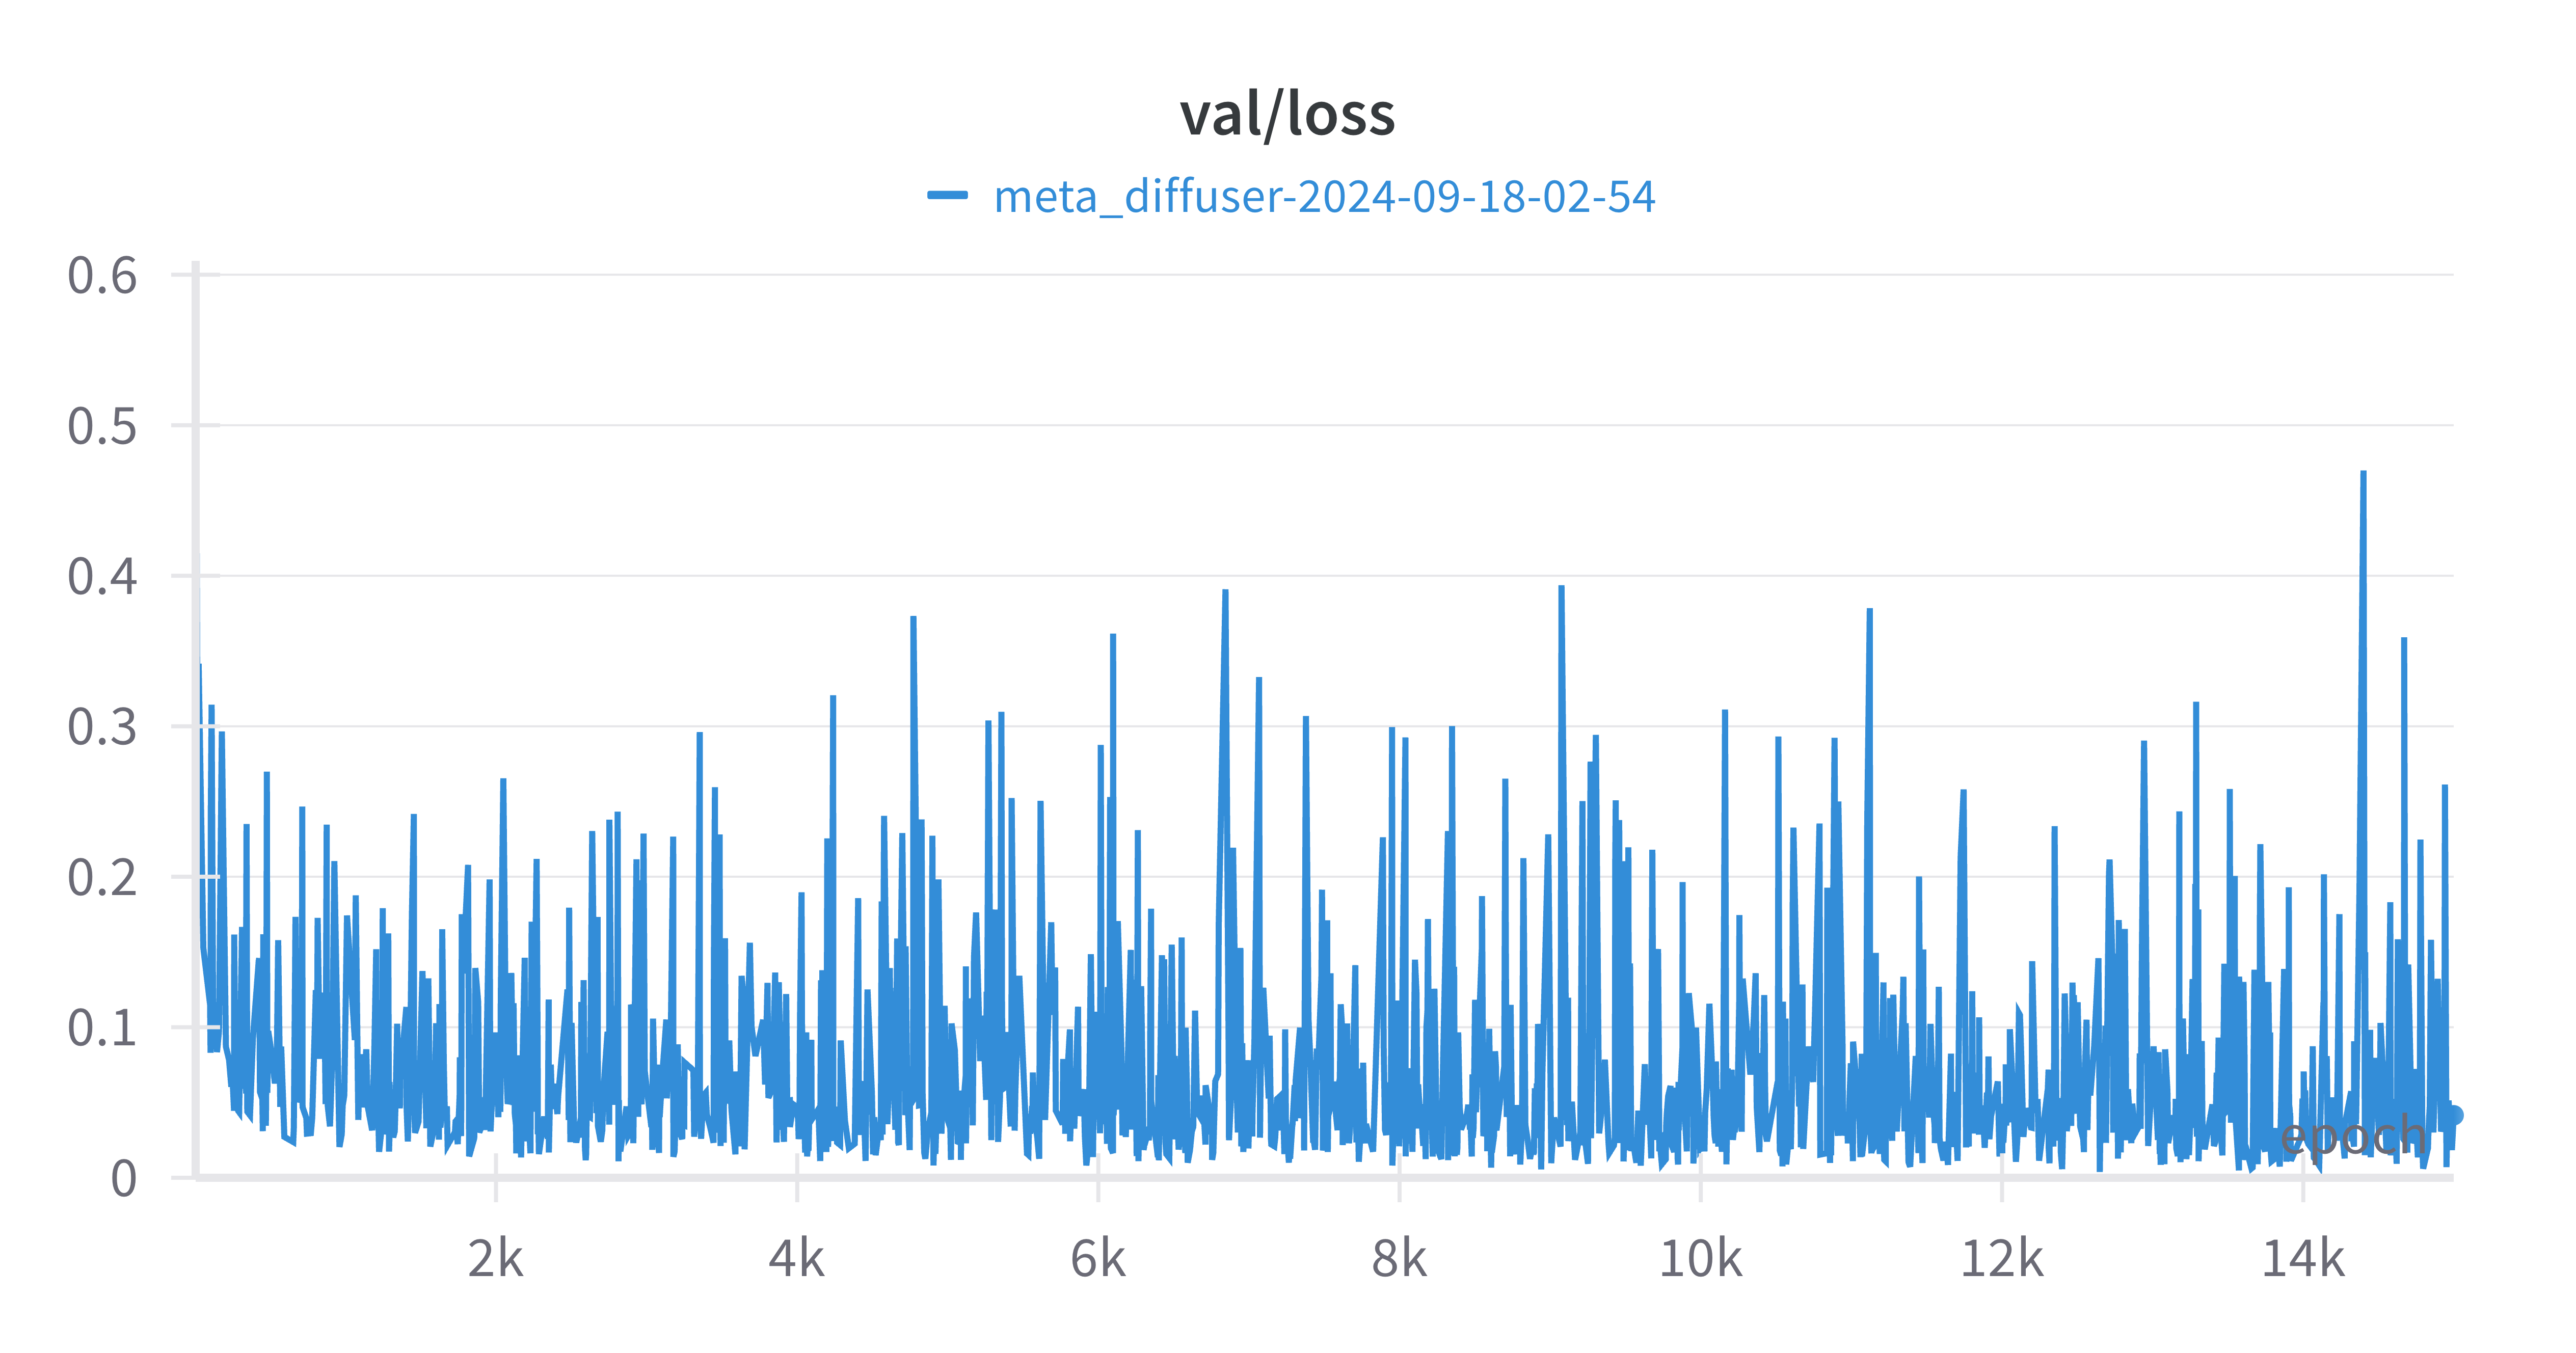
\includegraphics[width=\linewidth]{detailed_engineering/Meta Diffusion/charts/val_loss.png}
\caption{Loss during the validation. Lower is better.}
\endminipage
\end{figure}

Additional metrics evaluating the quality of the generated scan.
\begin{figure}[H]
\minipage{0.49\textwidth}
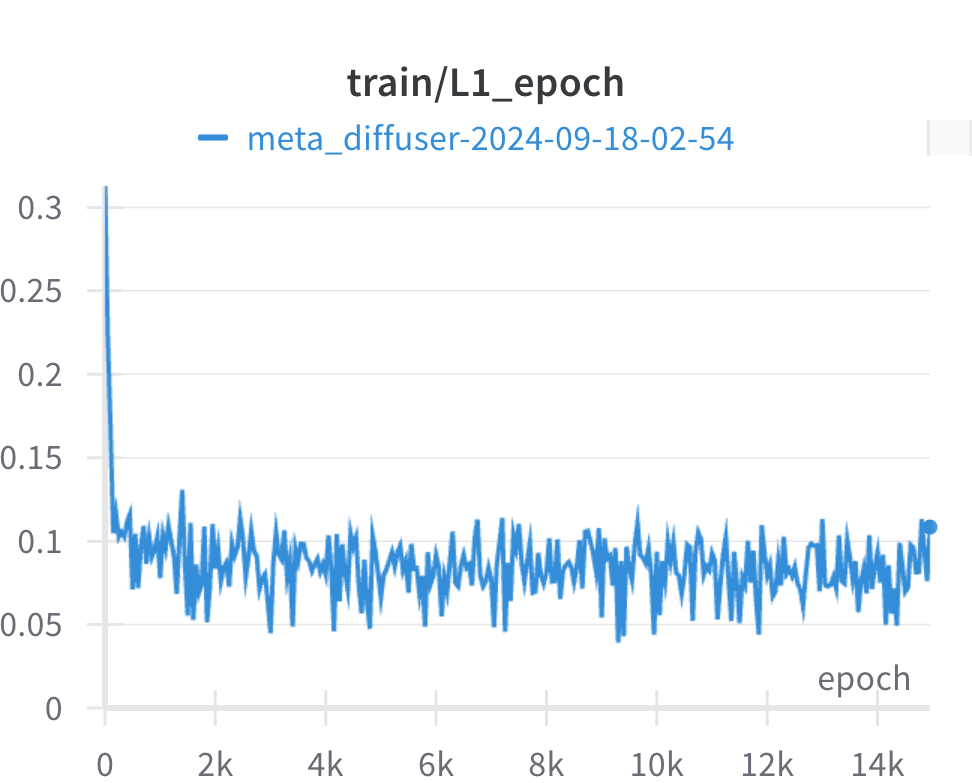
\includegraphics[width=\linewidth]{detailed_engineering/Meta Diffusion/charts/train_l1_epoch.png}

\endminipage\hfill
\minipage{0.49\textwidth}
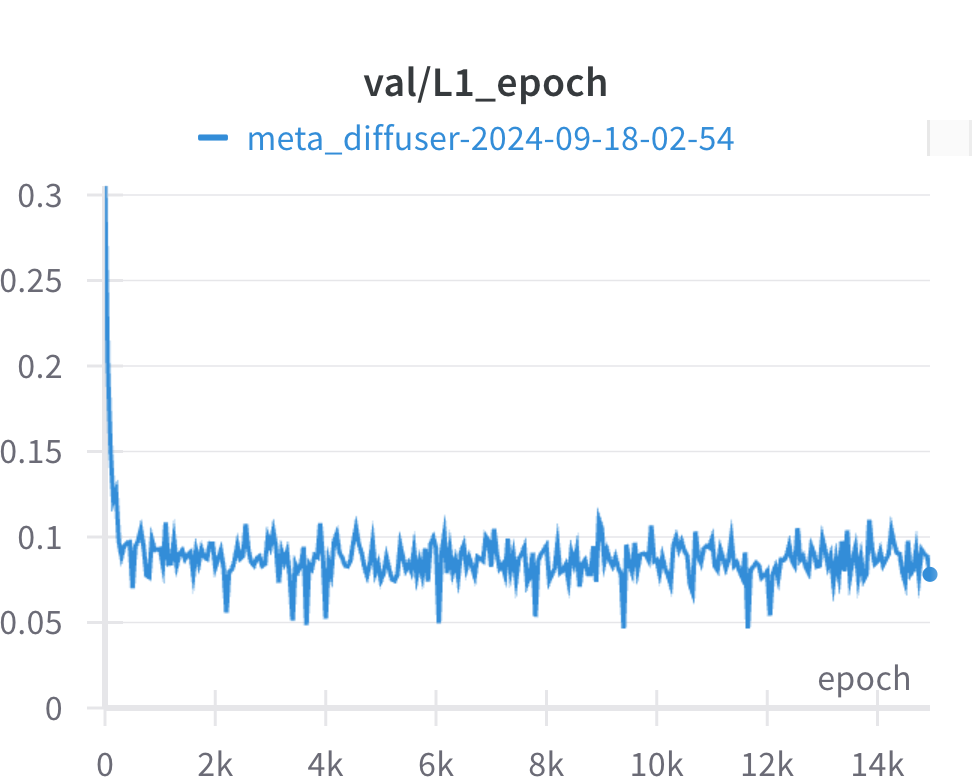
\includegraphics[width=\linewidth]{detailed_engineering/Meta Diffusion/charts/val_l1_epoch.png}

\endminipage
\caption{L1 between two generated CT scans and two random samples from training/validation datasets. Lower is better.}
\end{figure}

\begin{figure}[H]
\minipage{0.49\textwidth}
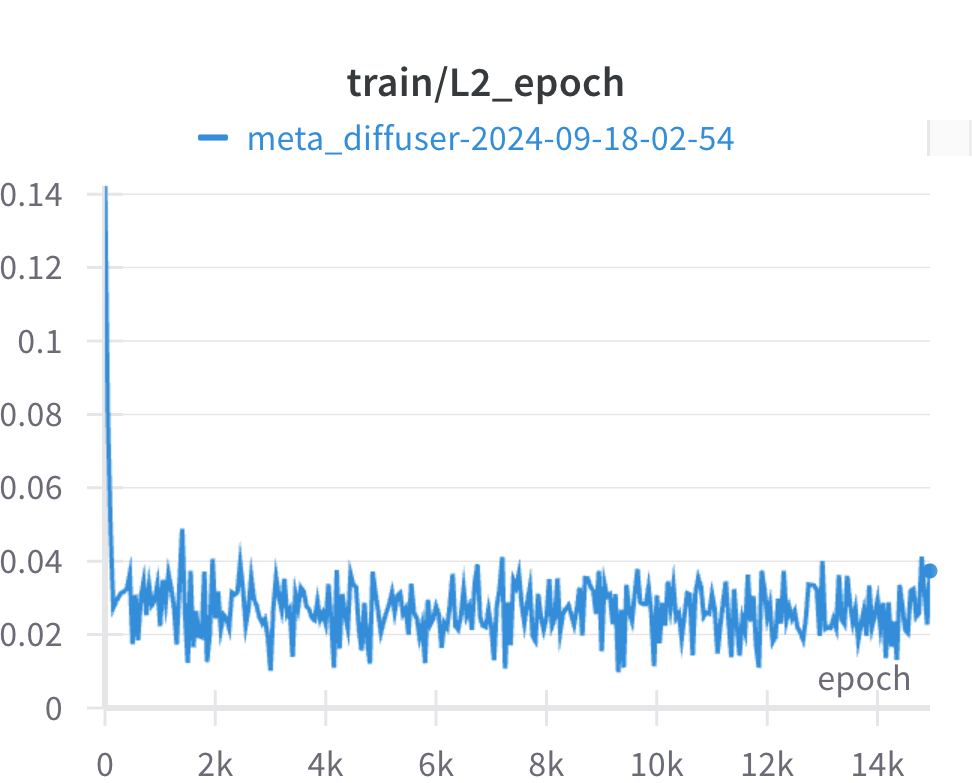
\includegraphics[width=\linewidth]{detailed_engineering/Meta Diffusion/charts/train_l2_epoch.png}

\endminipage\hfill
\minipage{0.49\textwidth}
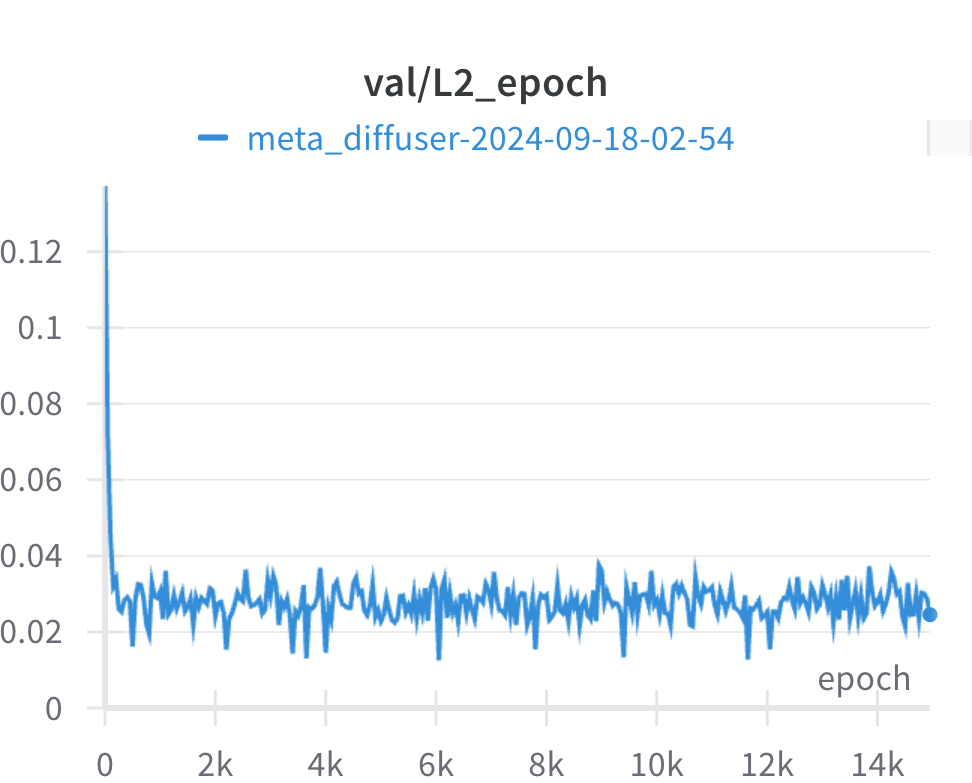
\includegraphics[width=\linewidth]{detailed_engineering/Meta Diffusion/charts/val_l2_epoch.png}

\endminipage
\caption{L2 between two generated CT scasn and two random samples from training/validation datasets. Lower is better.}
\end{figure}

\begin{figure}[H]
\minipage{0.49\textwidth}
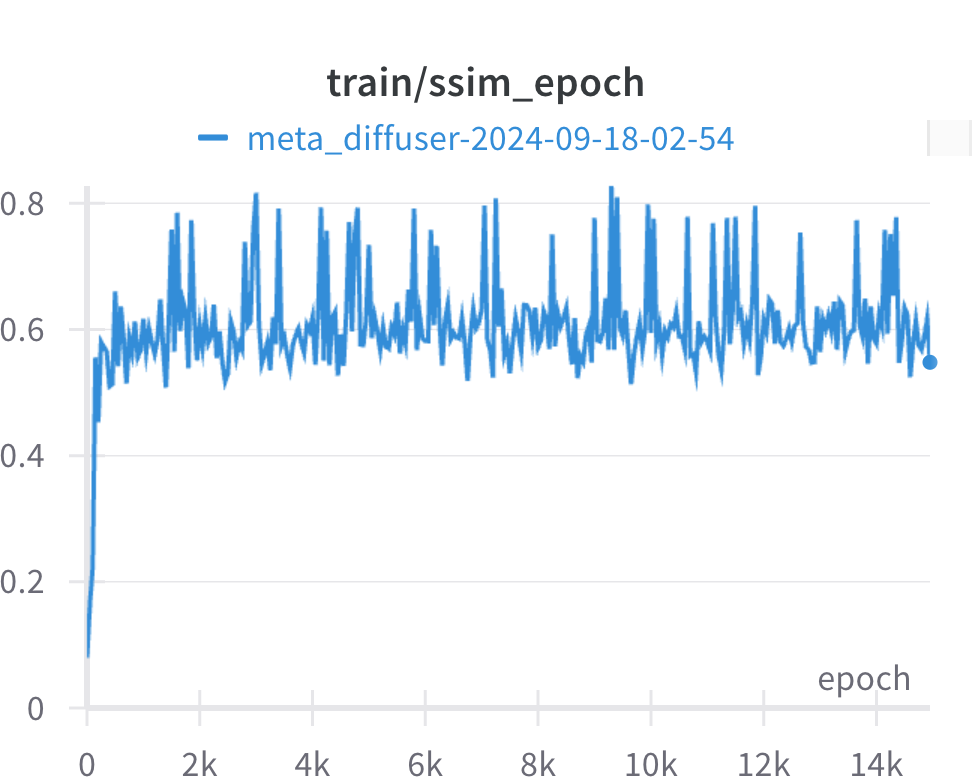
\includegraphics[width=\linewidth]{detailed_engineering/Meta Diffusion/charts/train_ssim_epoch.png}

\endminipage\hfill
\minipage{0.49\textwidth}
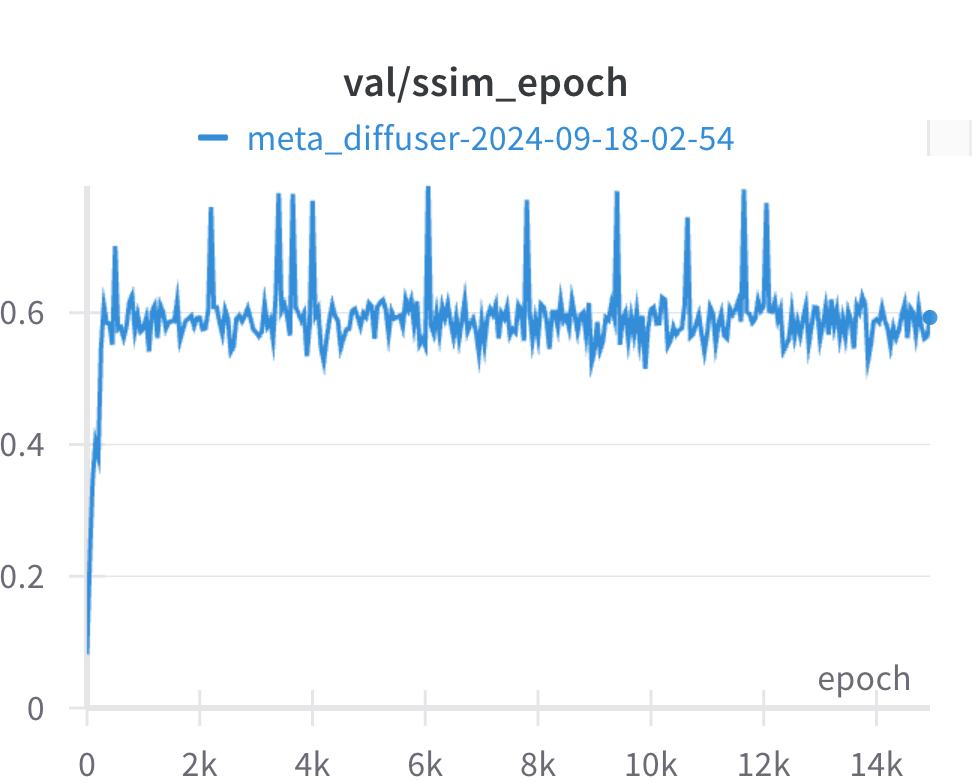
\includegraphics[width=\linewidth]{detailed_engineering/Meta Diffusion/charts/val_ssim_epoch.png}

\endminipage
\caption{MSSIM between two generated Ct scans and two random samples from training/validation datasets. Higher is better.}
\end{figure}

\paragraph{Results}\mbox{}\\

% \begin{figure}[H]
%     \centering
%     \includegraphics[width=\linewidth]{}
%     \caption{Caption}
%     \label{fig:enter-label}
% \end{figure}
\begin{figure}[H]
    \centering
    % \includegraphics{}
     \animategraphics[width=\textwidth, loop, autoplay]{5}%frame rate
    {detailed_engineering/Meta Diffusion/generation/layer-}%path to figures
    {0}%start index
    {31}%end index
    \caption{Random layer of synthetic CT scan generated from Gaussian noise.}
    \label{fig:my_label}
\end{figure}

\begin{figure}[H]
    \centering
    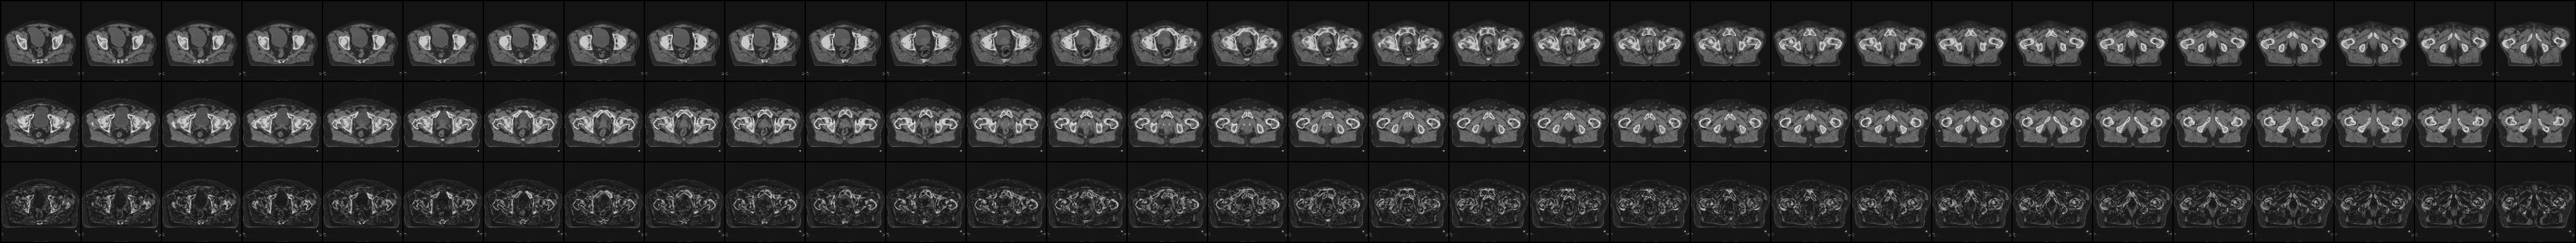
\includegraphics[width=\linewidth]{detailed_engineering/Meta Diffusion/charts/meta_diffusion_comparison.png}
    \caption{Top - first sample from trianing dataset, middle - synthetic CT scan, bottom - L1 difference between them.}
    \label{fig:ldm-success-comparison}
\end{figure}